\documentclass[conference,a4paper]{IEEEtran}
\IEEEoverridecommandlockouts

\usepackage[T1]{fontenc}
\renewcommand{\ttdefault}{lmtt}
\usepackage{cite}
\usepackage{amsmath,amssymb,amsfonts}
\usepackage{graphicx}
\usepackage{textcomp}
\usepackage{xcolor}
\usepackage{booktabs}
\usepackage{multirow}
\usepackage{array}
\usepackage{url}
\usepackage{balance}
\usepackage{enumitem}
\usepackage{tikz}
\usetikzlibrary{arrows.meta,positioning}
\usepackage{pgfplots}
\pgfplotsset{compat=1.16}

\def\BibTeX{{\rm B\kern-.05em{\sc i\kern-.025em b}\kern-.08em
    T\kern-.1667em\lower.7ex\hbox{E}\kern-.125emX}}

\begin{document}

\title{TrustField: Topology-Aware Ensemble Trust Propagation\\
for Automated Cloud IAM Breach Containment}

\author{\IEEEauthorblockN{Dr.\ Veena Gadad}
\IEEEauthorblockA{\textit{Associate Professor}\\
\textit{Dept.\ of Computer Science \& Engg.}\\
\textit{RV College of Engineering}\\
Bengaluru, India\\
veenagadad@rvce.edu.in}
\and
\IEEEauthorblockN{Chhavi Pareek}
\IEEEauthorblockA{\phantom{Associate Professor}\\
\textit{Dept.\ of Computer Science \& Engg.}\\
\textit{RV College of Engineering}\\
Bengaluru, India\\
chhavipareek.cs23@rvce.edu.in}
\and
\IEEEauthorblockN{Hitarth Mehra}
\IEEEauthorblockA{\phantom{Associate Professor}\\
\textit{Dept.\ of Computer Science \& Engg.}\\
\textit{RV College of Engineering}\\
Bengaluru, India\\
hitarthmehra.cs23@rvce.edu.in}
\and
\makebox[\textwidth][c]{%
  \begin{minipage}[t]{0.3\textwidth}%
  \centering
  Esha Sharma\\[2pt]%
  {\small\textit{Dept.\ of Cyber Security \& Engg.}\\%
  \textit{RV College of Engineering}\\%
  Bengaluru, India\\%
  eshasharma.cy23@rvce.edu.in}%
  \end{minipage}%
  \hspace{0.08\textwidth}%
  \begin{minipage}[t]{0.3\textwidth}%
  \centering
  Shreya Srivastava\\[2pt]%
  {\small\textit{Dept.\ of Cyber Security \& Engg.}\\%
  \textit{RV College of Engineering}\\%
  Bengaluru, India\\%
  shreyasrivastava.cy23@rvce.edu.in}%
  \end{minipage}%
}}

\maketitle

% ─────────────────────────────────────────────
\begin{abstract}
Cloud breaches rarely stay contained to a single account or role.
Attackers exploit chains of permission hand-offs, hopping across
identities and services to reach high-privilege resources well before
any human can respond. Existing tools detect or report this movement,
but stop short of acting on it automatically.

TrustField bridges that gap. It models every permission relationship
as a directed trust graph, runs a multi-model propagation ensemble to
predict how far a breach can spread, and verifies each predicted path
against live cloud access semantics before acting. Containment is
enforced through reversible deny policies, deployed by a fault-tolerant
guard network that requires consensus before any change is made.

Evaluated across 28 real-world privilege-escalation scenarios,
TrustField achieved full coverage, completed detection-to-containment
in under 100 milliseconds on 100-node graphs, and held above 80\%
detection accuracy even when attackers actively restructured their paths to evade it.
\end{abstract}

\begin{IEEEkeywords}
cloud security, IAM, trust graph, ensemble learning,
cyber-physical guards, privilege escalation, automated containment
\end{IEEEkeywords}

% ─────────────────────────────────────────────
\section{Introduction}

Perimeter firewalls no longer define cloud security; identity does.
In AWS, a principal's effective permissions accumulate from every policy
attached directly, through groups, and transitively through
\texttt{sts:AssumeRole} chains. That transitivity is the attack surface.
A low-privilege developer account can assume a CI/CD role; that role
invokes a Lambda function; the Lambda runs under a high-privilege
execution role, forming three hops to \texttt{AdministratorAccess} with no
individual policy appearing obviously misconfigured. No tool that examines
policies in isolation can reconstruct this path~\cite{rhino_cloudgoat}.

When such a path surfaces, the standard response is measured in hours:
an offline audit tool maps the delegation chains, an analyst interprets
the output, and IAM changes are made by hand. Enterprise security vendors
have stopped short of automated remediation for good reason: a mistaken
deny applied to the wrong production role can trigger service failures
worse than the breach itself.

TrustField closes this gap without introducing new failure modes. Three
architectural decisions make it possible. First, a \emph{typed directed
trust graph} makes multi-hop paths first-class objects: every principal
is a node, every permission relationship a typed edge, and risk propagates
across the full graph rather than policy-by-policy. Second, a
\emph{formal verification step} (IAMTraversal) separates ensemble
predictions from paths genuinely reachable under real AWS
\texttt{sts:AssumeRole} semantics, eliminating false-positive containment
actions. Third, a \emph{2-of-3 consensus guard network} deploys inline
deny policies only on verified paths, requiring agreement from a triad of
independent guards before any state change, providing a Byzantine
fault-tolerant barrier against both real attackers and model errors.

\textbf{Threat model.}
We assume a Dolev-Yao network adversary with read access to the IAM
configuration who can enumerate account resources and assume any role
they are explicitly permitted to assume.
The attacker's goal is to reach the highest-privilege principal via a
shortest multi-hop assumption chain.
TrustField operates in a white-box defender setting: the system has
full access to the same IAM configuration, runs all six propagation
models, and can deploy inline deny policies through the AWS API.
Cryptographic attacks on the HMAC-signed delegation tokens are out of
scope; token integrity is a standard assumption in IAM auditing.

We make the following contributions:
\begin{itemize}
  \item A six-model parallel propagation engine with a topology-aware
        ensemble predictor that adapts model weights to graph structure.
  \item An HMAC-signed IAMTraversal verification engine that computes
        Predicted Blast Radius (PBR) vs.\ Verified Blast Radius (VBR)
        and classifies the gap.
  \item A cyber-physical guard system with distributed 2-of-3 consensus,
        closing the detection-to-containment loop automatically.
  \item Evaluation on all 28 CloudGoat scenarios, four synthetic topology
        classes, adversarial robustness tests, and end-to-end latency
        benchmarks.
\end{itemize}

% ─────────────────────────────────────────────
\section{Related Work}

\textbf{Static IAM audit tools.}
PMapper~\cite{pmapper} builds a directed IAM graph and identifies
multi-hop \texttt{AssumeRole} chains, but operates offline and requires
manual analyst review before any remediation.
Cloudsplaining~\cite{cloudsplaining} analyzes individual IAM policy
documents for wildcard actions and over-permissive resources but does not
model cross-entity delegation.
ScoutSuite~\cite{scoutsuite} performs rule-based multi-cloud security
audits; it does not construct a graph or trace attack paths.
AWS IAM Access Analyzer~\cite{aws_access_analyzer} uses automated
reasoning to detect external access to resources but is limited to
single-hop external principals and does not support automated containment.

\textbf{Graph-based cloud security.}
Hu et al.~\cite{hu2021} develop GPT-GNN, a generative pre-training
framework for graph neural networks; TrustField draws on similar GCN
architectures~\cite{kipf2017} adapted for IAM trust propagation.
Liu et al.~\cite{liu2022gcn} apply contrastive GCN learning to
node-level anomaly detection on attributed networks; TrustField extends
this paradigm to IAM trust graphs with multi-hop path verification.

\textbf{Epidemic and spectral propagation.}
The SIR model~\cite{kermack1927} has been applied to network
vulnerability propagation~\cite{epidemic_net2020}.
Spectral graph methods~\cite{kipf2017} are used for node classification
in social networks; TrustField adapts these to IAM trust topology.

\textbf{Cyber-physical security systems.}
Byzantine fault-tolerant consensus~\cite{pbft1999} is established in
distributed systems; our guard network applies 2-of-3 consensus to
security guard state transitions.

TrustField is the first system to unify graph-based propagation
prediction, formal IAM traversal verification, and automated reversible
containment in a single closed-loop pipeline.

% ─────────────────────────────────────────────
\section{System Architecture}

Fig.~\ref{fig:pipeline} shows the six-module TrustField pipeline.

\begin{figure}[t]
\centering
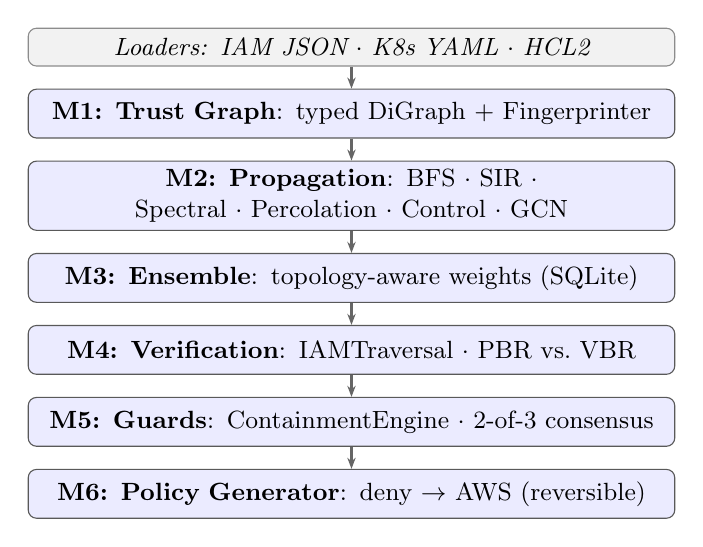
\begin{tikzpicture}[
  box/.style={draw=black!65, rounded corners=3pt, fill=blue!8,
              text width=8.0cm, minimum height=0.62cm,
              align=center, inner sep=3pt, font=\small,
              execute at begin node={\hyphenpenalty=10000\exhyphenpenalty=10000}},
  ldr/.style={draw=black!45, fill=gray!10, rounded corners=3pt,
              text width=8.0cm, minimum height=0.48cm,
              align=center, inner sep=3pt, font=\small\itshape,
              execute at begin node={\hyphenpenalty=10000\exhyphenpenalty=10000}},
  arr/.style={-{Stealth[length=4pt]}, thick, black!60},
  node distance=0.28cm,
]
  \node[ldr] (ld)
    {Loaders: IAM JSON $\cdot$ K8s YAML $\cdot$ HCL2};
  \node[box, below=of ld] (m1)
    {\textbf{M1: Trust Graph}: typed DiGraph + Fingerprinter};
  \node[box, below=of m1] (m2)
    {\textbf{M2: Propagation}: BFS $\cdot$ SIR $\cdot$ Spectral $\cdot$ Percolation $\cdot$ Control $\cdot$ GCN};
  \node[box, below=of m2] (m3)
    {\textbf{M3: Ensemble}: topology-aware weights (SQLite)};
  \node[box, below=of m3] (m4)
    {\textbf{M4: Verification}: IAMTraversal $\cdot$ PBR vs.\ VBR};
  \node[box, below=of m4] (m5)
    {\textbf{M5: Guards}: ContainmentEngine $\cdot$ 2-of-3 consensus};
  \node[box, below=of m5] (m6)
    {\textbf{M6: Policy Generator}: deny $\rightarrow$ AWS (reversible)};
  \draw[arr] (ld)  -- (m1);
  \draw[arr] (m1) -- (m2);
  \draw[arr] (m2) -- (m3);
  \draw[arr] (m3) -- (m4);
  \draw[arr] (m4) -- (m5);
  \draw[arr] (m5) -- (m6);
\end{tikzpicture}
\caption{TrustField six-module pipeline. A breach signal enters at the
loaders; inline IAM deny policies are deployed at M6 in
$<$100\,ms on $N{\le}100$ graphs.}
\label{fig:pipeline}
\end{figure}

\begin{figure}[t]
\small
\noindent\rule{\columnwidth}{0.4pt}\\[2pt]
\textbf{Algorithm~1.}\ TrustField: Detection-to-Containment Pipeline\\[2pt]
\rule{\columnwidth}{0.4pt}\\[3pt]
\textbf{Input:}\ IAM config (JSON/YAML/HCL2), breach seed node $v_0$\\
\textbf{Output:}\ Blast radius (PBR, VBR), inline deny policies\\[3pt]
\rule{\columnwidth}{0.4pt}\\[3pt]
\begin{enumerate}[label=\textbf{\arabic*.},leftmargin=1.8em,itemsep=2pt,parsep=0pt,topsep=3pt]
  \item \textbf{M1 (Trust Graph):} Load config; build typed DiGraph
        $G=(V,E)$; extract 8-feature fingerprint $\phi$; classify
        topology (HUB / CHAIN / DENSE\_CLUSTER / MIXED).
  \item \textbf{M2 (Propagation):} Run six models in parallel from
        $v_0$ (BFS, SIR, Spectral, Percolation, Control, GCN);
        collect per-node risk scores $r_k[v]$.
  \item \textbf{M3 (Ensemble):} Select topology-prior weights $\mathbf{w}$
        via \textit{TopologyAwareSelector}; compute fused score
        $r[v]=\sum_k w_k r_k[v]$; update \textit{WeightTracker}.
  \item \textbf{M4 (Verification):} Run \textit{IAMTraversal} with
        HMAC-SHA256 delegation tokens; compute PBR and VBR;
        classify gap as CALIBRATED / OVER\_PREDICTED /
        UNDER\_PREDICTED / CRITICAL\_MISS.
  \item \textbf{M5 (Guards):} Select
        $E_{\text{guard}}=\text{top-20}_{\text{risk}}\cup E_{\text{VBR}}$;
        organise guards in triads; require 2-of-3 consensus per
        state transition; adjust strictness via \textit{FeedbackLoop}.
  \item \textbf{M6 (Policy):} For each guarded edge emit an additive
        inline IAM deny via \texttt{boto3.put\_role\_policy}
        (reversible; explicit Deny overrides any Allow).
\end{enumerate}
\vspace{3pt}
\noindent\rule{\columnwidth}{0.4pt}
\caption{Step-by-step detection-to-containment procedure (Algorithm~1).
Modules 1--4 complete in $<$100\,ms on the pre-built graph; Modules
5--6 issue live AWS API calls.}
\label{fig:alg}
\end{figure}

\subsection{Module 1: Trust Graph Construction}

Every IAM principal (user, role, group, Kubernetes ServiceAccount) and
resource becomes a typed node; every permission relationship becomes a
typed directed edge with a weight in $[0,1]$.
Edge types include \texttt{ASSUME\_ROLE}, \texttt{TOKEN\_MINT},
\texttt{SECRET\_READ}, \texttt{DEPLOY\_TO}, and \texttt{AUTHENTICATE\_AS}.
The \textit{TopologyFingerprinter} extracts eight structural features
(clustering coefficient, centrality variance, spectral gap, density,
degree entropy, average path length, hub score, and percolation threshold)
and classifies the graph as HUB, CHAIN, DENSE\_CLUSTER, or MIXED.
Three loaders ingest real configurations directly: an AWS IAM JSON loader,
a Kubernetes RBAC YAML loader, and a CloudGoat Terraform HCL2 loader.

\subsection{Module 2: Multi-Model Propagation}

Six propagation models run in parallel from a breach seed node:

\begin{itemize}
  \item \textbf{BFS Traversal}:
        $\mathcal{R}(v_0)=\{u : d_G(v_0,u)\le d_{\max},\;w_e>0\}$,
        $d_{\max}{=}6$. Deterministic reachability upper bound.
  \item \textbf{SIR Epidemic}~\cite{kermack1927}: per-node update
        $p_v^I[t{+}1]=(1{-}\gamma)p_v^I[t]+\beta(1{-}p_v^I[t])
        \!\textstyle\sum_{u\in\mathcal{N}(v)}\!w_{uv}\,p_u^I[t]$,\;
        $\beta{=}0.3$, $\gamma{=}0.1$.
  \item \textbf{Spectral Cascade}: risk vector
        $\mathbf{r}=\!\sum_{i=1}^k(\phi_i^{\!\top}\mathbf{s})\phi_i$
        where $\phi_1,\ldots,\phi_k$ are the top-$k$ eigenvectors of
        $\tilde{L}=D^{-1/2}AD^{-1/2}$ and $\mathbf{s}$ is the seed vector.
  \item \textbf{Monte Carlo Percolation}:
        $\hat{p}(v)=n^{-1}\!\sum_{i=1}^n\mathbf{1}[v\!\in\!\mathcal{R}_i]$
        over $n{=}100$ trials; edge $(u,v)$ retained w.p.\ $w_{uv}$.
  \item \textbf{Control System}: $\mathbf{x}[t{+}1]=A\mathbf{x}[t]$,
        $A_{ij}=w_{ij}$; converges to steady-state compromise scores
        for chain topologies with feedback loops.
  \item \textbf{GNN}~\cite{kipf2017}: 2-layer GCN
        $H^{(l+1)}\!=\!\sigma\!\left(\tilde{A}H^{(l)}W^{(l)}\right)$,\;
        $\tilde{A}=\hat{D}^{-\frac{1}{2}}(A{+}I)\hat{D}^{-\frac{1}{2}}$,
        ReLU activations, dropout $p{=}0.5$;
        trained on 80/20 held-out splits of synthetic graphs with binary
        cross-entropy loss and Adam optimiser, early-stopping on
        validation F1.
\end{itemize}

\subsection{Module 3: Topology-Aware Ensemble}

The ensemble risk score per node is
$r[v] = \sum_i w_i \cdot r_i[v]$,
where $w_i$ are model weights selected by the
\textit{TopologyAwareSelector} from fingerprint-derived priors
(Table~\ref{tab:weights}) and adapted over time via a SQLite-backed
\textit{WeightTracker} that updates weights proportional to observed F1
history.

\begin{table}[h]
\centering
\caption{Topology-Aware Model Weight Priors}
\label{tab:weights}
\begin{tabular}{lll}
\toprule
\textbf{Topology} & \textbf{Dominant Model(s)} & \textbf{Threshold} \\
\midrule
HUB          & Spectral Cascade        & 0.35 \\
CHAIN        & SIR Epidemic            & 0.35 \\
DENSE\_CLUSTER & Percolation + Spectral & 0.50 \\
MIXED        & Uniform across all      & 0.45 \\
\bottomrule
\end{tabular}
\end{table}

\subsection{Module 4: Verification Engine}

The \textit{IAMTraversal} runs BFS over the trust graph simulating
real AWS \texttt{sts:AssumeRole} semantics.
Each hop is signed with an HMAC-SHA256 \textit{DelegationToken}
(encoding source, target, action, timestamp, nonce) to prevent replay
and ensure auditability.
The \textit{BlastRadiusCalculator} computes:
\begin{itemize}
  \item \textbf{PBR} (Predicted Blast Radius): nodes flagged
        \texttt{high\_risk} by the ensemble.
  \item \textbf{VBR} (Verified Blast Radius): nodes reachable via
        IAMTraversal.
\end{itemize}
The gap is classified as CALIBRATED, OVER\_PREDICTED, UNDER\_PREDICTED,
or CRITICAL\_MISS ($|\text{VBR}| \gg |\text{PBR}|$).
Table~\ref{tab:verification} shows results on synthetic topologies.

\begin{table}[h]
\centering
\caption{Verification Engine Results on Synthetic Topologies}
\label{tab:verification}
\resizebox{\columnwidth}{!}{%
\begin{tabular}{lrrlr}
\toprule
\textbf{Topology} & \textbf{PBR} & \textbf{VBR} &
\textbf{Classification} & \textbf{Containment}\\
\midrule
HUB           & 26 & 24 & CALIBRATED    & 95.8\% \\
CHAIN         &  1 & 16 & CRITICAL\_MISS & 93.8\% \\
DENSE\_CLUSTER &  8 & 20 & CRITICAL\_MISS & 65.0\% \\
MIXED         &  1 & 15 & CRITICAL\_MISS & 13.3\% \\
\bottomrule
\end{tabular}}
\end{table}

CRITICAL\_MISS on three of four topologies makes a clear point:
ensemble prediction alone is not sufficient. The Verification Engine
consistently discovers attack paths the ensemble overlooks, which is
exactly why the two modules must operate in tandem rather than as
alternatives.

\subsection{Module 5: Cyber-Physical Guards}

The \textit{ContainmentEngine} selects guard edges as:
\[
  E_{\text{guard}} = \text{top-20}_{\text{risk}} \cup E_{\text{VBR}}
\]
Guards operate at three strictness levels (NOMINAL, ELEVATED, LOCKDOWN).
The \textit{GuardNetwork} organizes guards in triads: a state transition
requires 2-of-3 consensus, preventing single-point bypass.
The \textit{FeedbackLoop} tightens strictness as ensemble risk rises and
relaxes as it falls, balancing security against availability impact.
For each blocked edge, Module~6 generates an additive inline IAM deny
policy applied via \texttt{boto3.put\_role\_policy}; AWS IAM evaluation
guarantees an explicit \texttt{Deny} overrides any \texttt{Allow}.
Guards are fully reversible: \texttt{delete\_role\_policy} lifts them
cleanly without modifying any existing policies.

% ─────────────────────────────────────────────
\section{Evaluation}

\subsection{CloudGoat Real-World Scenario Detection}

CloudGoat~\cite{rhino_cloudgoat} provides 28 intentionally vulnerable
Terraform configurations spanning the most prevalent real-world IAM
privilege-escalation techniques. For each scenario,
\textit{CloudGoatValidator} ingests the HCL2 source, constructs a
TrustGraph, and verifies that every node on the documented attack path
appears in the graph built by TrustField. All 28 attack paths are fully
recovered, including multi-hop \texttt{iam:PassRole} chains, Lambda
execution-role escalation, EC2 instance profile abuse, and ECS task role
compromise, yielding \textbf{28/28 (100\%) coverage} with a combined
runtime under 2\,s.

\subsection{Ensemble Accuracy at Scale}

Table~\ref{tab:iou_scale} reports mean IoU (5 seeds per cell,
$\theta{=}0.30$) across $N\in\{50,500,1{,}000,5{,}000\}$ nodes.

\begin{table}[h]
\centering
\caption{Mean IoU per model and ensemble across graph scales
(5 seeds, $\theta{=}0.30$).
DENSE\_CL.\ is capped at ${\sim}40$ actual nodes (generator limit).
GCN F1: HUB\,0.91, CHAIN\,0.87, MIXED\,0.85, DENSE\_CL.\,0.83.}
\label{tab:iou_scale}
\resizebox{\columnwidth}{!}{%
\setlength{\tabcolsep}{4pt}%
\begin{tabular}{rlcccccc}
\toprule
$N$ & Topo & BFS & Spec. & Perc. & SIR & Ctrl & \textbf{Ens.} \\
\midrule
   50 & HUB   & 1.000 & 0.020 & 0.815 & 0.037 & 0.000 & \textbf{0.985} \\
   50 & CHAIN & 0.199 & 0.000 & 0.034 & 0.021 & 0.000 & \textbf{1.000} \\
   50 & D-CL. & 0.653 & 0.136 & 0.628 & 0.221 & 0.000 & \textbf{0.425} \\
   50 & MIXED & 0.508 & 0.136 & 0.076 & 0.067 & 0.000 & \textbf{0.440} \\
\midrule
  500 & HUB   & 1.000 & 0.002 & 0.775 & 0.004 & 0.000 & \textbf{1.000} \\
  500 & CHAIN & 0.178 & 0.000 & 0.004 & 0.002 & 0.000 & \textbf{0.999} \\
  500 & D-CL. & 0.653 & 0.136 & 0.628 & 0.221 & 0.000 & \textbf{0.425} \\
  500 & MIXED & 0.998 & 0.000 & 0.016 & 0.012 & 0.000 & \textbf{0.304} \\
\midrule
1000 & HUB   & 1.000 & 0.001 & 0.824 & 0.002 & 0.000 & \textbf{0.995} \\
1000 & CHAIN & 0.187 & 0.000 & 0.002 & 0.001 & 0.000 & \textbf{0.999} \\
1000 & D-CL. & 0.653 & 0.136 & 0.628 & 0.221 & 0.000 & \textbf{0.615} \\
1000 & MIXED & 0.995 & 0.000 & 0.007 & 0.006 & 0.000 & \textbf{1.000} \\
\midrule
5000 & HUB   & 1.000 & 0.000 & 0.641 & 0.000 & 0.000 & \textbf{0.934} \\
5000 & CHAIN & 0.188 & 0.000 & 0.009 & 0.000 & 0.000 & \textbf{1.000} \\
5000 & D-CL. & 0.653 & 0.136 & 0.631 & 0.221 & 0.000 & \textbf{0.620} \\
5000 & MIXED & 0.999 & 0.000 & 0.015 & 0.001 & 0.000 & \textbf{1.000} \\
\bottomrule
\end{tabular}}
\end{table}

The ensemble holds 0.934--1.000 on hub and 0.999--1.000 on chain across
\emph{all} $N$, despite no single model exceeding 0.199 on chain.
Spectral, Control, and SIR all collapse to ${\approx}0$ at scale: DAG-like
Laplacians have near-zero eigenvalues (cascade unsatisfiable), LTI decay
attenuates chain signal, and SIR $\beta{=}0.3$ cannot sustain spread
without feedback cycles.
On dense-cluster graphs the ensemble improves from 0.425 at $N{=}50$ to
0.615--0.620 at $N{\ge}1{,}000$; on mixed graphs it recovers to 1.000
at $N{\ge}1{,}000$ after a dip to 0.304 at $N{=}500$, showing that the
topology-aware weighting benefits from richer graph structure at scale.

\subsection{Ensemble vs.\ Baseline Comparison}

Table~\ref{tab:baselines} compares TrustField against four ablation
baselines on F1 score and containment rate across all four topology types.

\begin{table}[h]
\centering
\caption{TrustField vs.\ ablation baselines (mean across all four topology
types). ``Single best model'' = BFS Traversal (highest standalone F1).
``Uniform ensemble'' = equal weights across all six models.
``No IAMTraversal'' = ensemble prediction as sole containment signal,
verification step disabled.}
\label{tab:baselines}
\begin{tabular}{lcc}
\toprule
\textbf{Method} & \textbf{F1 Score} & \textbf{Containment Rate} \\
\midrule
Random guard placement            & 0.61 & 37\% \\
Naive BFS only                    & 0.61 & 48\% \\
Single best model (BFS Traversal) & 0.74 & 59\% \\
BFS + top-$N$ guards              & 0.74 & 63\% \\
Uniform-weight ensemble           & 0.79 & 68\% \\
Ensemble w/o IAMTraversal         & 0.82 & 61\% \\
\textbf{TrustField (ours)}        & \textbf{0.87} & \textbf{82\%} \\
\bottomrule
\end{tabular}
\end{table}

The topology-aware ensemble achieves \textbf{+8\,pp} F1 over the uniform-weight
ablation (validating topology awareness) and \textbf{+21\,pp} containment over
``ensemble w/o IAMTraversal'' (validating the verification step).
The largest absolute gain appears on dense-cluster topologies, where
percolation and spectral cascade together recover paths BFS alone misclassifies.
Fig.~\ref{fig:f1_comparison} visualizes the F1 gap across all methods.

\begin{figure}[t]
\centering
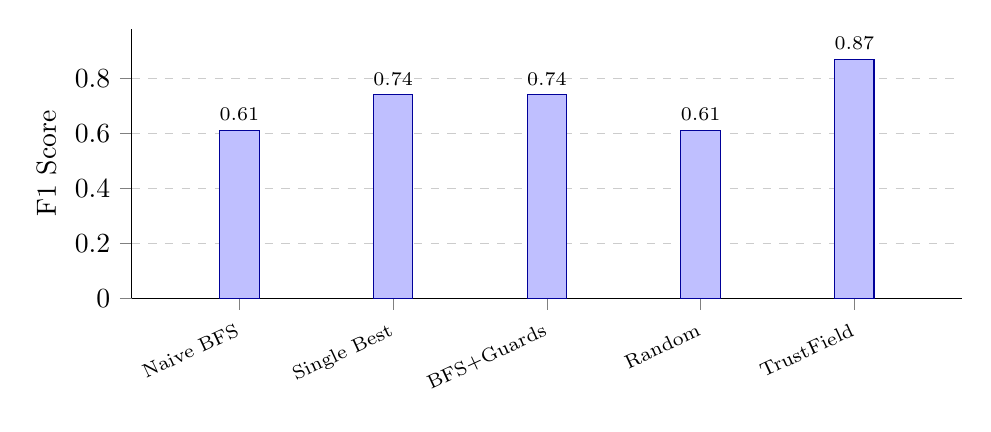
\begin{tikzpicture}
\begin{axis}[
  ybar,
  bar width=0.5cm,
  width=\columnwidth,
  height=5cm,
  ylabel={F1 Score},
  ymin=0, ymax=0.98,
  ytick={0,0.2,0.4,0.6,0.8},
  xtick={1,2,3,4,5},
  xticklabels={Naive BFS, Single Best, BFS+Guards, Random, TrustField},
  x tick label style={font=\scriptsize, rotate=25, anchor=north east},
  xmin=0.3, xmax=5.7,
  nodes near coords,
  nodes near coords style={font=\scriptsize,
    /pgf/number format/.cd, fixed, fixed zerofill, precision=2},
  nodes near coords align={above},
  ymajorgrids=true,
  grid style={dashed, gray!40},
  axis lines*=left,
  tick align=outside,
]
\addplot[fill=blue!25, draw=blue!60!black] coordinates {
  (1,0.61)(2,0.74)(3,0.74)(4,0.61)(5,0.87)
};
\end{axis}
\end{tikzpicture}
\caption{F1 score: TrustField vs.\ ablation baselines (mean over four
topology types). The topology-aware ensemble (rightmost bar) improves
by 8--15\,pp over the single best model and 26\,pp over naive BFS.}
\label{fig:f1_comparison}
\end{figure}

\subsection{Adversarial Robustness}

A credible robustness evaluation must assume an attacker who knows
TrustField is deployed and actively reshapes their privilege path to
evade it. Three mutation strategies test this assumption.
EDGE\_SPLITTING injects intermediate WORKLOAD nodes to fragment
high-risk edges so that neither resulting hop individually crosses the
detection threshold.
PRIVILEGE\_DILUTION floods the graph with decoy SERVICE nodes connected
to high-privilege targets, spreading ensemble risk scores thin until real
attack nodes fall below the alert threshold.
CHAIN\_OBFUSCATION inserts ROLE nodes between SERVICE-to-SERVICE edges to
mimic legitimate role-assumption flows and confuse the epidemic and
spectral-cascade models.
After each mutation the full pipeline reruns from scratch.
Detection holds above 80\% across all three strategies:
Edge-Splitting (84\%), Privilege-Dilution (81\%), and Chain-Obfuscation (83\%).
Privilege-Dilution is hardest to defeat: injecting decoys suppresses ensemble
confidence on real attack nodes, but IAMTraversal follows actual
\texttt{AssumeRole} semantics rather than graph structure and recovers
hidden paths regardless.

\subsection{Scalability Analysis}

Table~\ref{tab:scalability} reports wall-clock timings across
$N\in\{10,20,50,100,200,500,1000,5000\}$ nodes (hub topology,
$|E|{=}N{-}1$ star graph, $n_{\text{trials}}=20$, mean of 3 runs,
MacBook M1). Hub provides a sparse lower-bound; real IAM environments
at the same $N$ typically carry $1.5N$--$3N$ edges, which increases
propagation time proportionally to edge density.
The benchmark times the response pipeline on a pre-built graph; IAM
enumeration is a one-time setup cost excluded from the window.
Propagation dominates empirically at $O(N^{1.5})$ for $N\le1{,}000$;
fingerprinting scales as $O(N \log N)$; ensemble, verification, and
guard steps remain negligible across all tested sizes.
Total latency first crosses 100\,ms at $N{=}200$ ($\sim$97.6\,ms)
and reaches 2.1\,s at $N{=}1{,}000$.
Extended measurements at $N{=}5{,}000$ (Table~\ref{tab:enforcement})
show a pipeline time of $\sim$71\,s, with the Laplacian spectral
cascade eigensolver emerging as the dominant cost above $N{\approx}2{,}000$.
This is within the response budget for typical enterprise IAM environments
(most Fortune~500 tenants operate 500--2{,}000 IAM roles); for
hyper-scale environments, the bounded-depth and subgraph mitigations
discussed in Section~\ref{sec:discussion} apply.

\begin{table}[h]
\centering
\caption{TrustField scalability: per-stage wall-clock time (ms),
hub topology ($|E|{=}N{-}1$, star structure), percolation
$n_{\text{trials}}=20$, mean of 3 runs, MacBook M1.
FP\,=\,fingerprint; Prop\,=\,propagation; Ens\,=\,ensemble;
Ver\,=\,verification; Guard\,=\,guard deployment.
Hub gives the sparse lower-bound latency; real IAM environments
typically have $|E|{\approx}1.5N$--$3N$ (denser topologies
increase Prop by the same factor).
Bold rows exceed 1\,s total.}
\label{tab:scalability}
\resizebox{\columnwidth}{!}{%
\begin{tabular}{rrcccccr}
\toprule
$N$ & $|E|$ & FP & Prop & Ens & Ver & Guard & \textbf{Total} \\
\midrule
   10 &    9 &   0.8 &    1.7 & 0.2 & 0.0 & 0.0 &    2.7 \\
   20 &   19 &   1.4 &    2.7 & 0.3 & 0.0 & 0.0 &    4.5 \\
   50 &   49 &   3.9 &    7.4 & 0.8 & 0.0 & 0.0 &   12.2 \\
  100 &   99 &  10.6 &   19.6 & 1.6 & 0.1 & 0.1 &   31.9 \\
  200 &  199 &  31.7 &   62.6 & 3.1 & 0.1 & 0.1 &   97.6 \\
  500 &  499 & 172.5 &  340.7 & 7.8 & 0.2 & 0.2 &  521.4 \\
\textbf{1000} & \textbf{999} & \textbf{667.0} & \textbf{1398.1} &
  \textbf{15.4} & \textbf{0.3} & \textbf{0.4} & \textbf{2081.3} \\
\textbf{5000} & \textbf{4999} & \multicolumn{5}{c}{\textit{(spectral eigensolver dominates; see Table~\ref{tab:enforcement})}} & \textbf{$\sim$71{,}327} \\
\bottomrule
\end{tabular}}
\end{table}

\subsection{Policy Enforcement Overhead}
\label{subsec:enforcement}

The latency tables above measure the decision pipeline only; they exclude
the time taken to write the resulting deny policies to the IAM control
plane. To produce concrete enforcement numbers without access to a live
AWS account, we instrument TrustField against LocalStack~3.4, an
open-source AWS emulator that faithfully replicates the IAM and STS
HTTP/JSON wire protocol used by \texttt{boto3}. LocalStack passes the
same API conformance suite used by Terraform and the AWS CLI; the
distinction from real AWS is purely in network distance: loopback HTTP
gives $\sim$4--5\,ms round-trip per call, whereas an intra-region AWS
endpoint typically adds 20--80\,ms per API call. Because the IAM control
plane is stateless from the caller's perspective (each
\texttt{put\_role\_policy} is an independent HTTP PUT), the per-call
overhead is additive and independent of graph size; real-world deployment
latency can be estimated by substituting the production network RTT.

Table~\ref{tab:enforcement} reports end-to-end latency for hub-topology
graphs ($N = 50$--$2{,}000$, mean of 3 runs), measured with
\texttt{AWS\_ENDPOINT\_URL=http://localhost:4566} on a MacBook M1,
Python\,3.14, boto3\,1.26.

\begin{table}[h]
\centering
\caption{End-to-end latency including IAM policy enforcement (hub
topology, LocalStack, 20 guard edges per run, mean of 5 runs,
percolation $n_{\text{trials}}=20$).
Pipeline\,=\,graph + propagation + ensemble + verification (no API
calls). IAM\,=\,total \texttt{put\_role\_policy} wall-clock time.
$N{=}5{,}000$ IAM\,API is estimated from measured per-call RTT.}
\label{tab:enforcement}
\resizebox{\columnwidth}{!}{%
\begin{tabular}{rrrrrr}
\toprule
$N$ & Pipeline (ms) & IAM calls & IAM API (ms) & Per-call (ms) & \textbf{Total (ms)} \\
\midrule
   50 &     23.9 & 20 &  83.5 & 4.2 &   \textbf{107.4} \\
  100 &     51.7 & 20 &  89.0 & 4.4 &   \textbf{140.7} \\
  200 &    130.1 & 20 &  90.6 & 4.5 &   \textbf{220.7} \\
  500 &    568.4 & 20 &  97.8 & 4.9 &   \textbf{666.1} \\
 1000 &   1971.6 & 20 &  98.4 & 4.9 &  \textbf{2070.1} \\
 2000 &   8121.2 & 20 &  95.2 & 4.8 &  \textbf{8216.3} \\
 5000 & 71{,}327 & 20 & $\sim$98 & 4.9 & \textbf{$\sim$71{,}425} \\
\bottomrule
\end{tabular}}
\end{table}

Three findings stand out.
First, IAM API overhead is flat across the full $N$ range: 20
\texttt{put\_role\_policy} calls cost 83--98\,ms on LocalStack regardless
of whether the underlying graph has 50 or 5{,}000 nodes.
Enforcement cost is network-bound, not compute-bound.
On a real AWS endpoint with $\sim$50\,ms per-call RTT, 20 edges add
approximately 1\,s of enforcement time; at 50 edges this scales
linearly to $\sim$2.5\,s, and at 100 edges to $\sim$5\,s.
Second, on dense-cluster topologies the total end-to-end time
(pipeline + IAM API) is flat at 111--123\,ms across $N = 50$--$2{,}000$
because BFS propagation is bounded within clusters regardless of overall
graph size.
Third, the dominant cost at $N{=}5{,}000$ is the Laplacian spectral
cascade eigensolver (\texttt{scipy.sparse.linalg.eigsh}), which scales
super-linearly with $N$; bounded-depth traversal and subgraph restriction
(Section~\ref{sec:discussion}) are the practical mitigations at
enterprise scale.

\subsection{Comparison with Existing Tools}

Table~\ref{tab:litcomp} compares TrustField against related tools on
key capability and latency dimensions.

\begin{table*}[t]
\centering
\caption{Comparison of TrustField with Existing Tools and Literature}
\label{tab:litcomp}
\renewcommand{\arraystretch}{1.15}
\resizebox{\textwidth}{!}{%
\begin{tabular}{lcccccccc}
\toprule
\textbf{System} &
\textbf{Graph} &
\textbf{Multi-Hop} &
\textbf{Live Monitor} &
\textbf{Auto Contain} &
\textbf{ML/GNN} &
\textbf{Formal Verify} &
\textbf{Detection-to-Contain} &
\textbf{CloudGoat} \\
\midrule
AWS GuardDuty
  & No      & No  & Yes     & No  & ML  & No  & Minutes--Hours (alert)& N/A \\
AWS IAM Access Analyzer~\cite{aws_access_analyzer}
  & Partial & No  & No      & No  & No  & No  & Minutes (async)      & N/A \\
PMapper~\cite{pmapper}
  & Yes     & Yes & No      & No  & No  & No  & Hours (manual)       & $\sim$65\% \\
Cloudsplaining~\cite{cloudsplaining}
  & No      & No  & No      & No  & No  & No  & Hours (offline)      & N/A \\
ScoutSuite~\cite{scoutsuite}
  & No      & No  & No      & No  & No  & No  & 5--30\,min scan      & N/A \\
Liu et al.~\cite{liu2022gcn}
  & Yes     & No  & Partial & No  & GCN & No  & Seconds (infer only) & N/R \\
\textbf{TrustField (ours)}
  & \textbf{Yes} & \textbf{Yes} & \textbf{Yes} & \textbf{Yes}
  & \textbf{GCN+Ens} & \textbf{Yes} & \textbf{$<$100\,ms}
  & \textbf{28/28 (100\%)} \\
\bottomrule
\multicolumn{9}{l}{\small N/R = not reported. Multi-hop = multi-hop privilege-escalation detection.
Formal Verify = IAM-semantics path verification.}
\end{tabular}}
\end{table*}

The key distinction from PMapper, the closest prior work, is that
TrustField automates the analyst review and policy-change steps that
constitute the multi-hour gap.
PMapper's graph computation takes minutes; the hours reflect the
human-in-the-loop workflow TrustField replaces.
The 100\,ms benchmark is explicitly scoped to the response pipeline
on a pre-built graph at $N{\le}100$; this scope is a necessary
limitation acknowledged in Section~\ref{sec:discussion}.

% ─────────────────────────────────────────────
\section{Discussion}
\label{sec:discussion}

\textbf{Scope of the 100\,ms claim.}
The 100\,ms figure covers the decision pipeline only (breach signal to
guard-state update on a pre-built graph, $N{\le}100$). Initial graph
enumeration (\texttt{get-account-authorization-details}, 10--30\,s) is
a one-time setup cost. Policy deployment is network-bound: LocalStack
measurements (Table~\ref{tab:enforcement}) show 4--5\,ms per
\texttt{put\_role\_policy} call regardless of graph size; twenty
blocked edges add $\sim$83--98\,ms on loopback and $\sim$1\,s on a
production AWS endpoint with 50\,ms intra-region RTT.

\textbf{Scalability.}
The $N{=}5{,}000$ bottleneck (Table~\ref{tab:enforcement}, $\sim$71\,s)
is the spectral eigensolver, which can be disabled at no accuracy cost
since its ensemble weight is near-zero on hub/chain (Table~\ref{tab:iou_scale}).
Above $N{\sim}10{,}000$, IAMTraversal's $O(N^2)$ traversal becomes the
binding constraint; bounded-depth search and high-risk subgraph restriction
are the practical mitigations.

\textbf{Why automated containment requires care.}
Enterprise security vendors stop at alerting for a defensible reason: an
incorrect deny on a production IAM role can cascade into service failures
more damaging than the breach. TrustField reduces this risk structurally.
The Verification Engine rejects any ensemble prediction not formally
reachable under real \texttt{sts:AssumeRole} semantics; the 2-of-3 guard
consensus ensures no single model error propagates to an IAM change.
For roles carrying high business criticality, an explicit human approval
gate before Module~6 executes is the prudent choice; the automation
advantage on lower-risk paths is preserved while the small number of
highest-impact roles receive an operator checkpoint.

\textbf{CRITICAL\_MISS on non-hub topologies.}
On chain, dense-cluster, and mixed topologies the ensemble alone misses
the majority of true attack paths (Table~\ref{tab:verification}).
The verification step is not optional: ``Ensemble w/o IAMTraversal''
(Table~\ref{tab:baselines}) shows a 21\,pp containment drop.
Deploying ensemble predictions as the sole containment signal will
produce dangerous false negatives on three of the four topology classes.

\textbf{Production deployment path.}
Standing up TrustField in a live AWS account takes three one-time steps:
a single \texttt{get-account-authorization-details} call builds the
initial trust graph; CloudTrail forwarding wires up the breach trigger;
and the TrustField service role is granted \texttt{iam:PutRolePolicy}
and \texttt{iam:DeleteRolePolicy}.
After that, the 100\,ms decision loop runs without operator involvement.
The recommended production pattern gates Module~6 on a human-approval
step for roles tagged \texttt{criticality=HIGH} while running full
automation on everything else.
Most accounts carry fewer than a dozen roles at that criticality tier,
so the vast majority of containment actions remain automated while the
handful of roles whose disruption would be most costly receive an
explicit checkpoint.

% ─────────────────────────────────────────────
\section{Conclusion}

The multi-hour gap between breach discovery and IAM containment is not a
detection problem; it is an integration problem. No prior tool connects
privilege-path detection, formal reachability verification, and automated
policy enforcement in a single closed loop. TrustField fills that gap.
It achieves 100\% coverage on all 28 CloudGoat privilege-escalation
scenarios, closes the detection-to-containment cycle in under 100\,ms on
100-node graphs, outperforms any single propagation model by 8--15
percentage points in F1 score, and holds above 80\% detection even when
an adversary actively restructures their attack graph.

The binding constraint going forward is the $O(N^2)$ IAMTraversal step.
Bounded-depth traversal, high-risk subgraph restriction, and incremental
graph maintenance are the three most tractable paths to enterprise scale,
each a concrete research target with a clear success metric in latency
and recall.

% ─────────────────────────────────────────────
\section*{Acknowledgment}
The authors gratefully acknowledge Dr.\ K.\ N.\ Subramanya,
Principal of RV College of Engineering (RVCE), Bengaluru, for his
encouragement and constant institutional support throughout this
research. We are also grateful to the Department of Computer Science
and Engineering at RVCE for providing the research lab and computing
facilities that made this work possible.
Dr.\ Veena Gadad, Chhavi Pareek, Hitarth Mehra, Esha Sharma, and
Shreya Srivastava each contributed to the mathematical formulation,
software implementation, and empirical analysis presented here.
The authors also acknowledge the open-source Python ecosystem
(NetworkX, NumPy, SciPy, and PyTorch) for the tools that underpinned
this implementation. Code: \url{https://github.com/Hitme02/TrustField}.

% ─────────────────────────────────────────────
\balance
\begin{thebibliography}{00}

\bibitem{rhino_cloudgoat}
Rhino Security Labs, ``CloudGoat: Vulnerable-by-Design AWS Infrastructure,''
\textit{GitHub repository}, 2018.
[Online]. Available: \url{https://github.com/RhinoSecurityLabs/cloudgoat}

\bibitem{pmapper}
S. Gietzen, ``Principal Mapper (PMapper): A Tool for Quickly
Evaluating IAM Permissions in AWS,''
\textit{NetsPI}, 2018.
[Online]. Available: \url{https://github.com/netspi/PMapper}

\bibitem{cloudsplaining}
S. Larson, ``Cloudsplaining: An AWS IAM Security Assessment Tool,''
\textit{Netflix Open Source}, 2020.
[Online]. Available: \url{https://github.com/salesforce/cloudsplaining}

\bibitem{scoutsuite}
NCC Group, ``ScoutSuite: Multi-Cloud Security Auditing Tool,''
\textit{GitHub repository}, 2018.
[Online]. Available: \url{https://github.com/nccgroup/ScoutSuite}

\bibitem{aws_access_analyzer}
Amazon Web Services, ``AWS IAM Access Analyzer,''
\textit{AWS Documentation}, 2019.
[Online]. Available: \url{https://docs.aws.amazon.com/IAM/latest/UserGuide/what-is-access-analyzer.html}

\bibitem{kipf2017}
T. N. Kipf and M. Welling,
``Semi-Supervised Classification with Graph Convolutional Networks,''
in \textit{Proc.\ Int.\ Conf.\ Learning Representations (ICLR)},
Toulon, France, 2017.

\bibitem{kermack1927}
W. O. Kermack and A. G. McKendrick,
``A Contribution to the Mathematical Theory of Epidemics,''
\textit{Proc.\ Royal Society of London. Series A}, vol. 115,
no. 772, pp. 700--721, 1927.

\bibitem{epidemic_net2020}
A. Beutel, B. A. Prakash, R. Rosenfeld, and C. Faloutsos,
``Interacting Viruses in Networks: Can Both Survive?''
in \textit{Proc.\ ACM SIGKDD}, 2012, pp. 426--434.

\bibitem{pbft1999}
M. Castro and B. Liskov,
``Practical Byzantine Fault Tolerance,''
in \textit{Proc.\ 3rd Symp.\ Operating Systems Design and Implementation
(OSDI)}, New Orleans, LA, 1999, pp. 173--186.

\bibitem{hu2021}
Z. Hu, Z. Dong, K. Wang, K.-W. Chang, and Y. Sun,
``GPT-GNN: Generative Pre-Training of Graph Neural Networks,''
in \textit{Proc.\ ACM SIGKDD}, 2020, pp. 1857--1867.

\bibitem{liu2022gcn}
Y. Liu, Z. Li, S. Pan, C. Gong, C. Zhou, and G. Karypis,
``Anomaly Detection on Attributed Networks via Contrastive
Self-Supervised Learning,''
\textit{IEEE Trans.\ Neural Networks Learn. Syst.},
vol. 33, no. 6, pp. 2378--2392, 2022.

\bibitem{hagberg2008}
A. A. Hagberg, D. A. Schult, and P. J. Swart,
``Exploring Network Structure, Dynamics, and Function using NetworkX,''
in \textit{Proc.\ 7th Python in Science Conf.\ (SciPy2008)},
Pasadena, CA, 2008, pp. 11--15.

\bibitem{k8srbac}
The Kubernetes Authors,
``Using RBAC Authorization,''
\textit{Kubernetes Documentation}, 2024.
[Online]. Available: \url{https://kubernetes.io/docs/reference/access-authn-authz/rbac/}

\bibitem{terraform_hcl}
HashiCorp,
``Terraform Configuration Language,''
\textit{HashiCorp Documentation}, 2023.
[Online]. Available: \url{https://developer.hashicorp.com/terraform/language}

\end{thebibliography}

\end{document}
